\chapter[Introduction]{Scientific landscape}
\label{Chap:scientificLandscape}
\epigraph{``If you wish to create a Universe from scratch, the final ingredient would be clusters of galaxies.''}{— [Afiq Hamid 2025]}
\section{Galaxy Clusters}\label{Chap:scientificLandscapeGalaxyClusters}
It has been said that mass and time are among the most fundamental parameters in all of astrophysical science. This thesis is principally an exploration of the former through the study of the most massive gravitationally bound structures in the Universe: galaxy clusters. 
\pbreak
Galaxy clusters occupy a unique position within the hierarchy of astrophysical structures. They represent the endpoint of cosmic structure formation, populating the nodes that connect the filaments of the cosmic web \textcolor{red}{[ref]}. The matter composition of galaxy clusters is dominated by a hitherto enigmatic, collisionless dark matter (DM) component ($\sim80\%$), while the remaining baryonic constituents are made up of the intracluster medium (ICM), a diffuse and turbulent plasma ($\sim15\%$), with the luminous member galaxies — themselves home to most of the stars, planets, and people (human or otherwise) within the cluster  — make up the smallest residual ($\sim5\%$) \textcolor{red}{[ref]}.

Structurally the DM component dictates the overall potential well, setting the stage for all of the baryonic interactions \textcolor{red}{[ref]}. At the base of this immense potential well sits the largest galaxy known as the brightest cluster galaxy (BCG), that accounts for $0.5$--$2\%$ of the cluster baryons. BCGs commonly hosts an active galactic nucleus (AGN), a powerful source of energetic feedback attributed to super massive black hole (SMBH) activity as the origin \textcolor{red}{[ref]}. Understanding AGN physics is of broad interest in modern astrophysics, spanning diverse research areas from exotic accretion processes to high powered jet emission \textcolor{red}{[ref]}, \textcolor{red}{[ref]}, and while not the primary focus of this work, AGN feedback has major implications towards the stirring of gas motions within the ionised ICM.

Permeating the space between the member galaxies in a cluster is the ICM. It is a hot ($T \sim 10^7$--$10^8$ K), diffuse ($n_e \sim 10^{-3}$--$10^{-1}$ cm$^{-3}$), optically thin, volume-filling plasma. The ICM is threaded by a weak but dynamically relevant magnetic field ($\sim1$--$10\,\mu$G), detectable via Faraday rotation measures \textcolor{red}{[ref]}. As the primary atmosphere of the cluster, the ICM plays an important role in various dynamical processes therein.

\begin{itemize}
	\item \textbf{\textit{AGN thermostat}} The ICM regulates the cooling of gas towards the cluster core — a process that, if left unchecked, would produce excess star formation rates (SFR) in the BCG. In the absence of a heating mechanism, the dense core would radiate energy efficiently and cool on timescales far shorter than the cluster age, driving a so-called cooling flow \textcolor{red}{[ref]}. This cooling is now understood to be moderated by a self-regulating feedback loop: as gas cools and accretes onto the BCG it fuels the central AGN, which injects energy back into the ICM via jets and lobes, suppressing further cooling of the core regions \textcolor{red}{[ref]}. The ICM therefore acts as both the fuel supply and calorimeter of this baryonic cycle.
	\item \textbf{\textit{Star formation in member galaxies}} The ICM plays an influential role on the evolutionary life-cycle tracks and SFR of its member galaxies through quenching mechanisms and ram-pressure stripping (RPS). As the satellite galaxies fall into the cluster potential well, contact with the ICM removes internal cold gas reservoirs from the interstellar medium (ISM) of the galaxies, quenching star formation on relatively short timescales ($t \sim 0.3$ Gyr) \textcolor{red}{[ref]}. This is most evident on close approach to the core and manifests as the stripped tails of jellyfish galaxies \textcolor{red}{[ref]}. Conversely, on longer timescales ($t \sim 3$ Gyr) strangulation targets the outer hot gas halo and prevents new gas from cooling \textcolor{red}{[ref]}, \textcolor{red}{[ref]}.
	\item \textbf{\textit{Cluster mass bias}} Cluster mass measurements can be used as cosmological probes of the large scale matter distribution of the Universe constraining several important parameters of the \LCDM cosmology model \textcolor{red}{[ref]}. Since the DM component cannot be directly observed by any present means, the ICM provides a useful observational marker to constrain cluster masses via complementary multi wavelength approaches. However, the approaches are heavily dependent on the assumption that the ICM gas exists in a state of quiescent hydrostatic equilibrium (HE) within the DM potential well \textcolor{red}{[ref]},\textcolor{red}{[ref]}. 	
\end{itemize}

The observational leverage acquired on all three of the aforementioned processes is mediated through how the ICM manifests across the electromagnetic spectrum. The next section details the primary observational windows through which the ICM is studied in order to derive constraints on cluster mass, and sets the groundwork for the key physical quantities and input assumptions that underpin the contents of the later chapters.

\newpage
\section{Observables}\label{Chap:scientificLandscapeObservables}

Optical light as the oldest astronomical window was used to initially identify and catalog the first galaxy groups and clusters \textcolor{red}{[Abell 1958]}. It remains a viable way to evaluate the matter content of galaxy clusters via gravitational lensing \textcolor{red}{[Kneib \& Natarajan 2011]} and velocity dispersion of member galaxies  \textcolor{red}{[Girardi et al. 1998]}. However, the windows of most relevance toward understanding the thermodynamic properties of the ICM exist on opposite ends of the electromagnetic spectrum: namely, the X-ray and millimeter-wave radio.

\subsection{X-ray emission}\label{Chap:scientificLandscapeObservablesXray}

The X-ray window played a vital role in the initial discovery and characterisation of the ICM. The ICM of galaxy clusters remain among the brightest X-ray sources in the sky to date \textcolor{red}{[ref]}. The emission is predominantly produced via thermal bremsstrahlung (free-free emission), in which electrons are deflected by ions and radiate photons in the process. The X-ray surface brightness $S_\mathrm{X}$ of the ICM electrons is proportional to the line-of-sight (LOS) emission integral:

\begin{equation}
	S_\mathrm{X} \propto \int n_e n_p \, \Lambda(T) \, \mathrm{d}l 
	\approx \int n_e^2 \, \Lambda(T) \, \mathrm{d}l,
	\label{eq:Sx}
\end{equation}
\\
where $n_e$ and $n_p$ are the electron and proton number densities respectively, $\Lambda(T)$ is the plasma cooling function. Since the emissivity scales as $n_e^2$, X-ray probes ICM gas density and in combination with grazing-incidence, total external reflection optics provides high resolution studies of the ICM core. However, this sensitivity can be a double-edged sword as the $n_e^2$ dependence means that $S_\mathrm{X}$ can be biased by an unknown gas clumping factor arising from inhomogeneity in the core \textcolor{red}{[ref]}.
\pbreak
Since the sound crossing time (represented by the time it takes for pressure fluctuations to travel across a region in the ICM)  within an Abell radius of 3 Mpc is only 0.17 - 0.33 of the Hubble time (the timescale of the cluster formation and evolution), it is generally assumed that the ICM will eventually settle into a state of approximate HE where pressure forces counter act against gravity:

\begin{equation}
	\frac{1}{\rho_g}\frac{dP}{dr} = -\frac{d\phi}{dr} = 
	-\frac{GM(<r)}{r^2},
	\label{eq:HE}
\end{equation}
\\
where $M(<r)$ is the total mass enclosed within the spherically symmetric radius $r$, $\phi$ is the gravitational potential, $\rho_g$ is the gas density, and $P$ is pressure. This balance of forces is the gas-phase expression of the clusters's broader virialized state and provides a foundational framework through which X-ray observations can be used to infer cluster mass.  Idealised hydrodynamic-simulation tests of the HE assumption show some useful agreement with true cluster mass, with RMS scatter of 15 $\%$ within the central few Mpc but growing mildly with radius, and can balloon locally to a factor of two in the presence of shocks or unrelaxed substructure  \textcolor{red}{[Schindler 1996]} \textcolor{red}{[ref]}. %\textcolor{blue}{However, there are some limitations of the X-ray method that can be complemented by other wavelengths.}

\newpage
Another important concept that emerged from the X ray regime is the analytical $\beta$-model. By applying an approximation for a self-gravitating collisionless system to a radial model of gas distribution in equilibrium within the same potential \textcolor{red}{[Cavaliere \& Fusco-Femiano 1976]} derived the analytic isothermal radial $\beta$ model of the ICM electron number density:

\begin{equation}
n_{gas}(r) = n_0 \left[ 1 + \left( \frac{r}{r_c} \right)^2 \right]^{-\frac{3}{2}\beta},
	\label{eq:3DradialBeta}
\end{equation}
\\
where $n_0$ is the central gas number density, $r_{c}$ is the radius of the cluster core and the index $\beta \sim 2/3$ is known as the canonical $\beta$ value \textcolor{red}{[ref]}. The profile describes a flat central core transitioning to a power-law decline at large radii. Its broad applicability across the cluster population follows naturally from the self-similar nature of galaxy clusters. While modern high-resolution observations and hydrodynamical simulations have revealed limitations of the model — particularly in its inability to capture asphericities from complex merging and dynamically disturbed systems — it remains a robust and widely used first approximation for the ICM radial gas density distribution \textcolor{red}{[ref]}. 

\subsection{Radio Sunyaev-Zel’dovich effect}\label{Chap:scientificLandscapeObservablesRSZ}

The thermal Sunyaev--Zel'dovich effect (tSZ) is a secondary anisotropy of the cosmic microwave background (CMB)  arising from the inverse Compton scattering of CMB photons by hot thermal electrons within the ICM \textcolor{red}{[Sunyaev \& Zel'dovich 1970]}, \textcolor{red}{[Sunyaev \& Zel'dovich 1972]}. As CMB photons traverse the cluster, a small fraction are energetically upscattered, producing a characteristic frequency dependent spectral distortion  given by:
%a decrement in CMB intensity at frequencies $\nu < 217$ GHz and a corresponding increment at $\nu > 217$ GHz. The resulting distortion in CMB intensity is :

\begin{equation}
	\Delta I_{\nu} = y \frac{2 h \nu^{3}}{c^{2}} \frac{x e^{x}}{(e^{x} - 1)^{2}} \left[ x\frac{ e^{x} + 1   }{e^{x} - 1} - 4  \right],
	\label{eq:Distortion}
\end{equation}
\\
where $x = h\nu/k_BT$ is the dimensionless frequency, 
$T = 2.725$ K is the CMB temperature, $h$ is Planck's 
constant, and $k_B$ is Boltzmann's constant. The amplitude of the distortion is set by the Compton $y$ parameter, which is proportional to the LOS integral of the electron pressure:

\begin{equation}
	y = \frac{\sigma_{T}}{m_{e}c^{2}} \int P_{e} dl,
	\label{eq:comptony}
\end{equation}
\\
where $P_{e} = n_{e}k_{B}T$ and $\sigma_{T}$ is the Thomson cross section. The Compton $y$ parameter therefore provides a direct in-situ measure of the integrated thermal pressure of the cluster along the LOS. A key advantage of the tSZ signal over $S_{X}$ is its linear dependence on electron density making it more sensitive to the low-density outskirts of the cluster towards the virial radius. Coupled with a sufficiently wide field of view (FOV), the tSZ effect is therefore more suited to mapping the thermodynamic structure of the ICM on large scales and by shows promise in mapping the cosmic baryon distribution \textcolor{red}{[Mroczkowski2019]}. Figure \ref{fig:multispectralComa} shows a multispectral image of the Coma cluster of galaxies combining both tSZ and $S_{\mathrm{X}}$.

\begin{figure}[p]
	\vspace*{\fill}
	\begin{center} 
		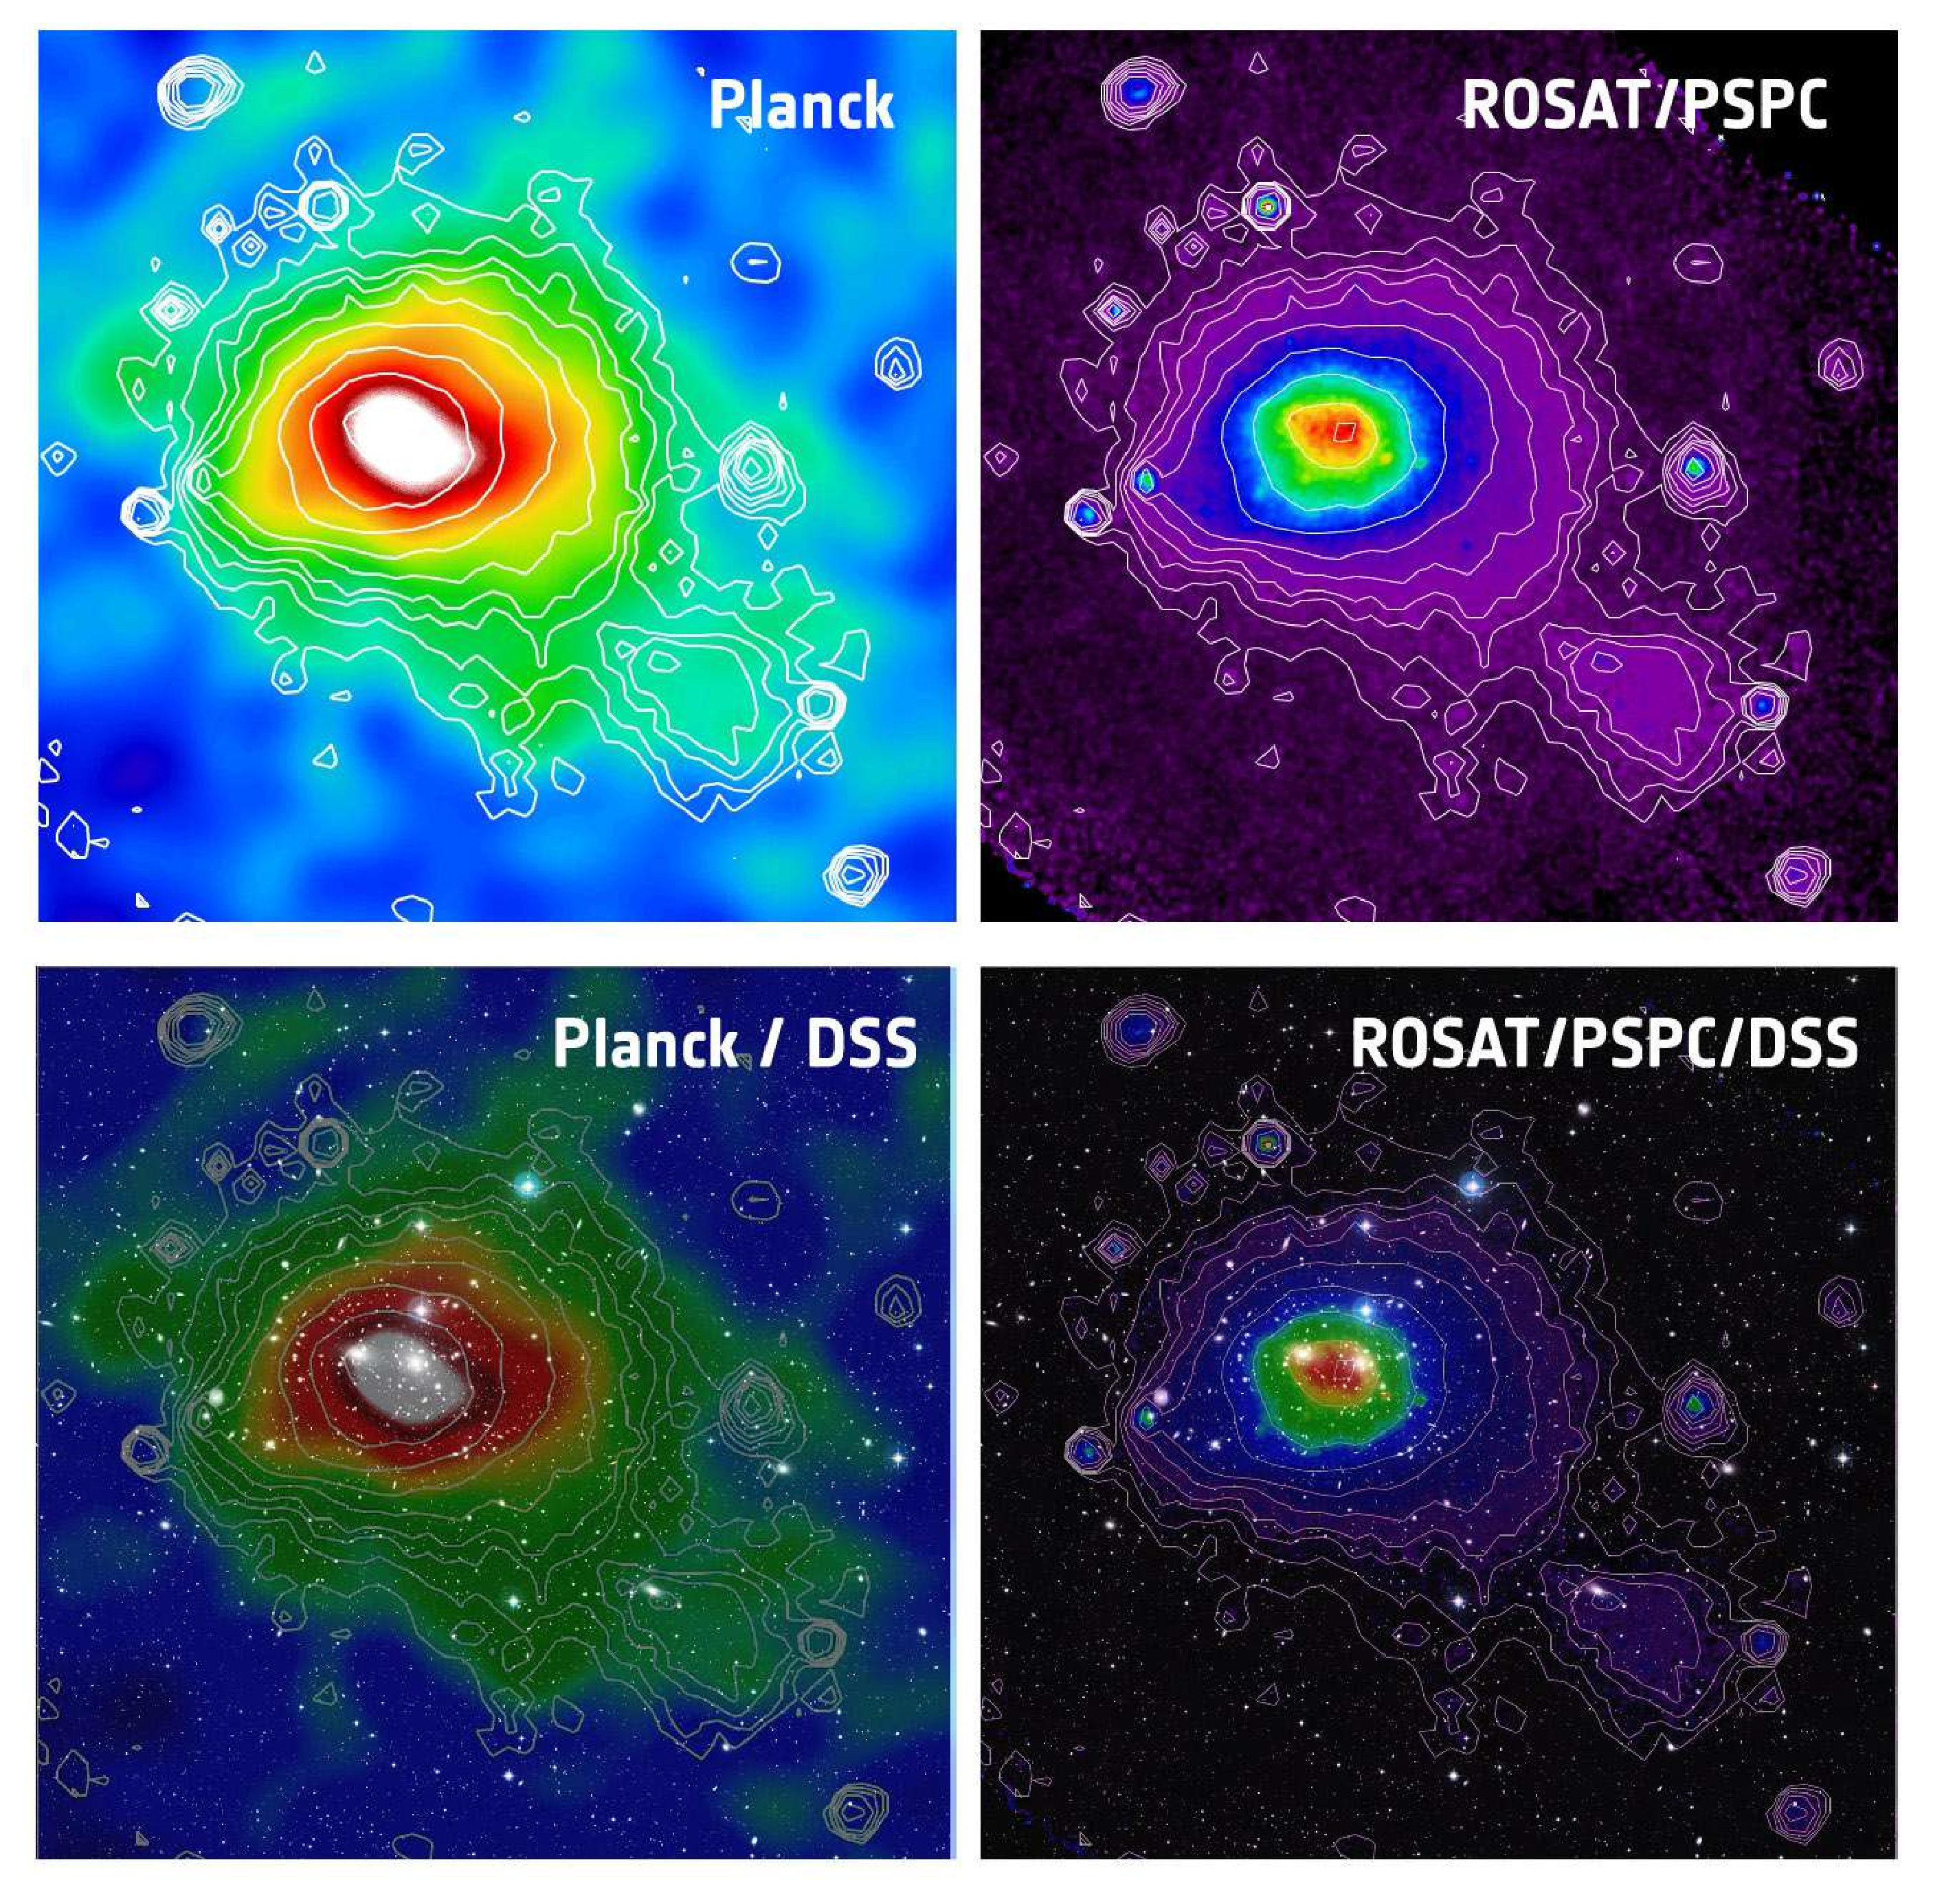
\includegraphics[width=1.0\textwidth]{Chapter1/imgs/1567218868444-COMA_ROSATvsPLANCK.pdf}
		\caption{Multiwavelength composite of the Coma cluster (Abell 1656). Top left: Planck tSZ Compton $y$ map. Top right: ROSAT soft X-ray surface brightness. In both upper panels the X-ray contours are superimposed on the tSZ image to illustrate the complementary spatial coverage of the two windows. The primary difference between the two regimes is that the tSZ emission is more spatially extended while the X-ray image is more centrally peaked. The bottom panels show the mult spectral image overlaid on the optical image, further revealing the member galaxy distribution. \textcolor{red}{[ref]} \textcolor{red}{[ref]}.}
		\label{fig:multispectralComa}
    \end{center}
\vspace*{\fill}
\end{figure}

\section{ICM structure and non-thermal pressure}\label{Chap:scientificLandscapePhysicalSourceTurb}

Notwithstanding the overview provided thus far, the ICM is in reality a complex and dynamically evolving system. The true gas conditions are in actuality far removed from the idealised equilibrium state assumed prescribed by \ref{eq:HE}. A truer conceptual picture — one favoured in the present literature — models the ICM as a stratified, multiphase fluid confined by the cluster potential but dynamically governed by a combination of thermal and non-thermal processes.  \textcolor{red}{[Donahue \& Voit 2022]}\textcolor{red}{[Battaglia et al. 2012]}. This section briefly interrogates each of these ideas in further detail.

\subsubsection{A fluid description of the ICM}

The treatment of the ICM as a fluid is suitable when the mean free path $\lambda_\mathrm{mfp}$ of the constituent particles is much smaller compared to the characteristic scale length $L$ of the system. For the bulk ICM, $\lambda_\mathrm{mfp} \approx 4.6$ kpc \textcolor{red}{[ref]}, which is well below the scales of interest for cluster-wide gas dynamics — justifying the use of the Euler or Navier--Stokes equations as a fluid description \textcolor{red}{[ref]}. However, this fluid approximation is not universal. In the low-density outskirts of clusters, where the mean free path is much higher, and on small scales where kinetic plasma effects become important, a purely hydrodynamic description breaks down and kinetic or magnetohydrodynamic (MHD) formulisms are more appropriate \textcolor{red}{[ref]}.

\subsubsection{Stratification}

Stratification implies that there is a radial ordering of the different thermodynamic properties — principally density, temperature, and entropy all under the simultaneous influence of gravity \textcolor{red}{[ref]}. The condition of stratification is characterized by the Brunt--V\"{a}is\"{a}l\"{a} (BV) frequency:

\begin{equation}
	N_\mathrm{BV}^2 = \frac{g}{\gamma}\frac{d}{dr}\ln{\frac{P}{\rho_{\mathrm{g}}^{\gamma}}},
	\label{eq:BrutVaisalaFreq}
\end{equation}
\\
where $g$ is the local gravitational acceleration, $\gamma$ is the adiabatic index, $P$ is the thermal pressure, $\rho$ is the gas density, and $r$ is the radial coordinate. The quantity $P/\rho^\gamma$ is proportional to the specific entropy $K$, thus $N_\mathrm{BV}^2$ also describes an entropy gradient. When $N_\mathrm{BV}^2 > 0$ — as is generally the case throughout the bulk ICM where entropy increases outward — the stratification is stable: a radially displaced gas parcel experiences a restoring buoyancy force and oscillates about its equilibrium position at frequency $N_\mathrm{BV}$ rather than convecting freely. This suppresses radial mixing while also supporting the propagation of internal gravity waves ($g$-modes) which are themselves a carriers of turbulent energy \textcolor{red}{[ref]}. \textcolor{blue}{There are some edge cases that exist beyond the purely hydrodynamic cases that can introduce exotic processes such as magneto thermal instabilities (MTI) which argue for conditions that could prove degenerative to these stable $N^2$ state \textcolor{red}{[ref]}. In this case what happens?}

\subsubsection{Multiphase structure}

The ICM is also not characterised by a single thermal phase. Modern observations and simulations reveal a multiphase environment in which gas spans a wide range of temperatures — from cold molecular filaments at $T \lesssim 10^2$ K to the bulk hot phase at $T \sim 10^{7}$--$10^{8}$ K \textcolor{red}{[ref]}. This stands in sharp contrast to the traditional picture of a uniform hot atmosphere, and draws analogy to the multiphase structure of the more local ISM.
\pbreak
Cold phases and filaments in the ICM develop as a result of thermal instability and chaotic cold accretion (CCA) \textcolor{red}{[ref]}. The CCA process within cluster cores is analogous to precipitation: where the local cooling time drops below the free-fall time, allowing for gass to condense out of the hot phase and gravitationally accrete onto the center as cold filaments and clouds \textcolor{red}{[ref]}. A key theoretical challenge of understanding this turbulent process is trying to figure out how the cold filaments are not evaoprated back into the hot phase \textcolor{red}{[ref]}. The current candidates are a mix of anisotropic thermal conduction, unique magnetic field alignments, and heat flux buoyancy instabilities (HBI).

\subsection{Non-thermal pressure}
Within the stratified, multiphase fluid described of the ICM a range of dynamical phenomena occur that challenge the HE assumption. These challenges come in the form of bulk motion, turbulence, cosmic rays, and magnetic fields that all contribute non-thermal pressure components. In reality, the total pressure support within the ICM is not provided by thermal component alone:

\begin{equation}
	P_\mathrm{tot} = P_\mathrm{th} + P_{\mathrm{nt}} = P_\mathrm{th} + \frac{1}{3}\rho_{\mathrm{g}}\sigma_v^{2},
	\label{eq:Ptot}
\end{equation}
\\
where $\sigma_{v}$ is the velocity dispersion of isotropically moving gas decomposable into radial and tangential components \textcolor{red}{[ref]}. Random turbulence and ordered gas motions contribute the most dominant part of $P_\mathrm{NT}$, with cosmic rays and magnetic fields contributing only at the level of a few per cent \textcolor{red}{[ref]}. From comparisons between theory and observation, residual gas motions are estimated to contribute between $\sim 10\%$ at $R_{500}$ and $\sim 30\%$ at $R_{200}$ of the total pressure support, with this fraction increasing in dynamically disturbed systems 
\textcolor{red}{[ref]}.
\pbreak
Constraining $P_\mathrm{nt}$ observationally is a non-trivial 
problem. Direct constraints are in principle accessible through 
X-ray spectroscopy, with velocity broadening and shifts of spectral emission line methods \textcolor{red}{[ref]}\textcolor{red}{[ref]}. However, the spatial coverage of current X-ray spectroscopic instruments is limited, and the technique is restricted to relatively nearby, X-ray bright systems as a result of cosmological dimming. The radio SZ surface brightness fluctuation methods investigated in this work offer a spatially extended alternative, at the cost of a greater number of modeling assumptions — the characterization and interrogation of which are attempted throughout the next two chapters.

\subsection*{Astrophysical sources of ICM gas motions.}
\label{Chap:scientificLandscapeSourcesGasMotions}

The non-thermal pressure within clusters is sustained via continuous injection of kinetic energy into the ICM. The injection originates from a hierarchy of physical drivers operating across a wide range of spatial scales \textcolor{red}{[ref]}. These can be broadly ordered from large to small as follows.
\pbreak
On the largest scales, the dominant energy source is gravitational — energy enters the system through the hierarchical assembly of large-scale structure through major cluster mergers and the continuous accretion of unvirialized material along cosmic web filaments \textcolor{red}{[ref]}. Major mergers between clusters of comparable mass drive powerful shocks and large-scale bulk flows that inject kinetic energy on scales approaching the virial radius, with the resulting turbulence taking of order a Gyr to equilibriate. Figure \ref{fig:merging_clusters} presents a gallery of merging clusters to illustrate the phenomenon. %Evidence from simulations shows the   $P_{\mathrm{th}}$ to $P_{NT}$ fraction rising up to $30\%$ in the outskirts near $R_{200}$ \textcolor{red}{[ref]}. 
\pbreak
On intermediate scales, minor mergers and glancing interactions on the scale of galaxy groups drive sloshing motions that set the cluster atmosphere into coherent oscillations without fully disrupting the cool core \textcolor{red}{[ref]}. These produce cold fronts — sharp contact discontinuities between the displaced cool core gas and the surrounding hotter ICM — visible as edges in $S_{\mathrm{X}}$ \textcolor{red}{[ref]}. The sloshing flows are indicated to be subsonic corresponding to velocities of several hunder kilometres per second and mach numbers in the range of 0.3-0.5 \textcolor{red}{[ref]}. The infall of dark matter subhaloes further stirs the ICM on scales intermediate between the merger and core scales, contributing gaseous wakes from RPS and turbulent substructure \textcolor{red}{[ref]}.
\pbreak
On the smallest scales, AGN feedback injects mechanical energy directly into the cluster core via jets and radio-mode outflows, inflating cavities visible in $S_{\mathrm{X}}$ and driving weak shocks that propagate outward into the surrounding ICM \textcolor{red}{[ref]}. The buoyantly rising cavities transfer most of their energy to the gas after crossing several pressure scale heights of the atmosphere \textcolor{red}{[ref]}. Additional contributions arise from plasma instabilities — including MTI and HBI — that operate in the weakly magnetised ICM and can drive small-scale anisotropic turbulent motions, particularly in the cluster outskirts \textcolor{red}{[ref]}.
\pbreak
The cumulative effect of this multi-scale energy injection is a turbulent velocity field and fluctuations that permeates the ICM from the virial radius inward. In the next section we consider some of the fundamental physical attributes of the turbulence phenomena are explored.  

\clearpage
\begin{figure}[p]
	\vspace*{\fill}
	\centering
	
	% Row 1
	\begin{tabular}{cc}
		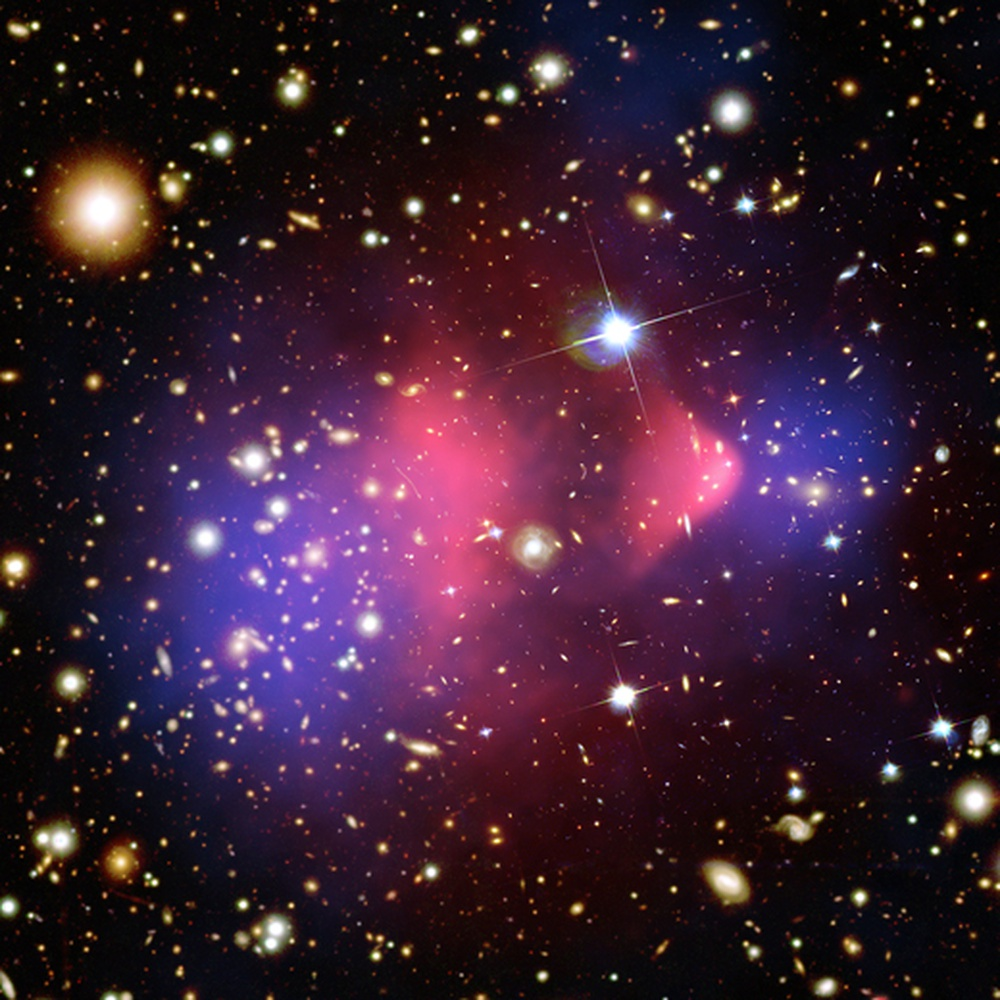
\includegraphics[width=0.42\textwidth, 
		height=0.42\textheight, 
		keepaspectratio=true]
		{Chapter1/imgs/clusters/bulletCluster_sq.jpg}
		&
		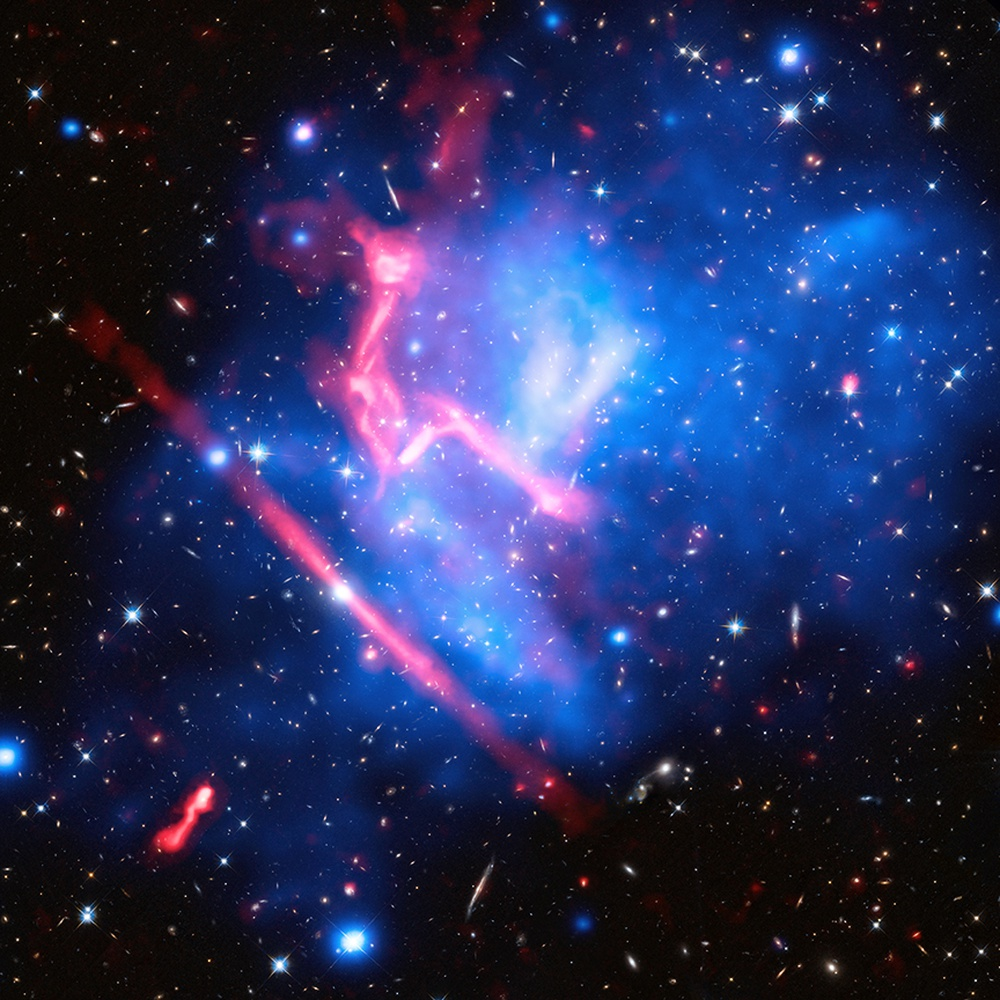
\includegraphics[width=0.42\textwidth, 
		height=0.42\textheight, 
		keepaspectratio=true]
		{Chapter1/imgs/clusters/Macsj0717_sq.jpg}
		\\[0.5em]
		% Row 2
		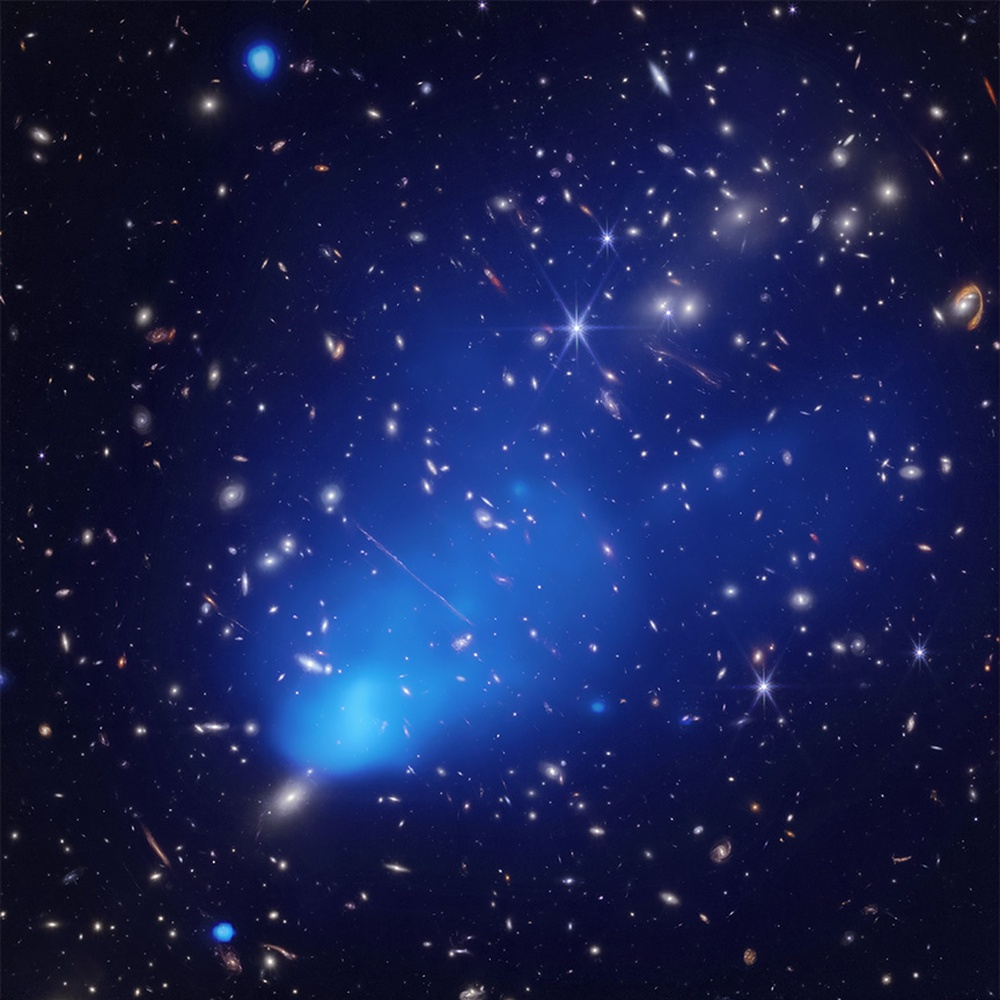
\includegraphics[width=0.42\textwidth, 
		height=0.42\textheight, 
		keepaspectratio=true]
		{Chapter1/imgs/clusters/elgordoCluster_sq.jpg}
		&
		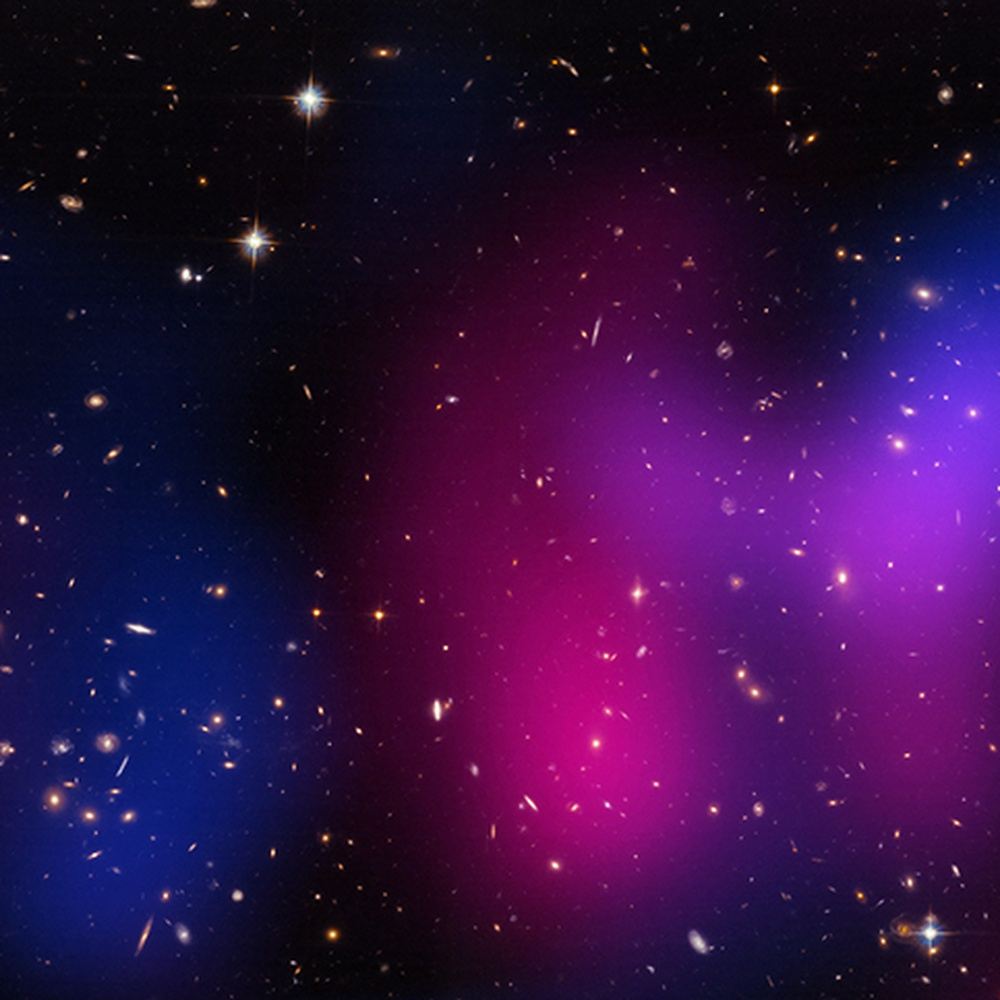
\includegraphics[width=0.42\textwidth, 
		height=0.42\textheight, 
		keepaspectratio=true]
		{Chapter1/imgs/clusters/musketBall_sq.jpg}
		\\
	\end{tabular}
	%\caption{Spectacular merging clusters. The bullet, MACS, ElGordo, MusketBall }
	\caption{A gallery of dynamically disturbed galaxy clusters representing extreme violations of hydrostatic equilibrium. \textit{Top left:} The Bullet Cluster (1E~0657-56), the archetypal binary merger. Chandra X-ray emission (pink) traces the shocked ICM stripped from the collisionless dark matter (blue, lensing reconstruction), providing the first direct observational evidence for dark matter.\textcolor{red}{[ref]}. \textit{Top right:} MACS~J0717.5+3745, the result of a 	quadruple cluster collision fed by a 13~Mpc cosmic web filament.Chandra X-ray (blue), VLA radio (red), and HST optical (background) reveal an extraordinarily complex thermodynamic structure \textcolor{red}{[ref]}. \textit{Bottom left:} El Gordo (ACT-CL~J0102-4915), the most 	massive known merging cluster at $z \sim 0.87$. Chandra X-ray emission (blue) is overlaid on a JWST infrared composite, with gravitational lensing arcs visible in the background field \textcolor{red}{[ref]}. \textit{Bottom right:} The Musket Ball Cluster (DLSCL~J0916.2+2951), a post-merger system caught further along in its evolution than the Bullet Cluster. The clear spatial offset between the hot gas (red) and dark matter (blue) illustrates the different collisional cross-sections of baryonic and dark matter \textcolor{red}{[ref]}.}
	\label{fig:merging_clusters}
	\vspace*{\fill}
\end{figure}
\clearpage
\section{Turbulence theory}\label{Chap:scientificLandscapeTurbulenceTheory}

Turbulence is the study of irregular, chaotic fluid motion — one of the oldest unsolved problems in classical physics because of the non linear nature of its fundamental equations. In the terrestrial context it governs everything from the drag on aircraft wings to the mixing of cream in coffee. In the astrophysical context, the problem becomes even richer and more challenging: the characteristic scales incredibly vast with no well-defined boundaries, the fluid is self-gravitating, and the turbulence unfolds within a plasma intimately coupled to magnetic fields, and continuous energy injection from mergers and accretion. The ICM represents one of the most extreme turbulent environments in the Universe, and the true nature of its turbulent velocity field remains an open question in modern astrophysics.
\pbreak
The fundamental condition that allows for the onset turbulence is set by the Reynolds number:

\begin{equation}
	\mathrm{Re} = \frac{u l_\mathrm{inj}}{\nu},
	\label{eq:reynolds}
\end{equation}
\\
where $u$ is the characteristic velocity of the flow, $l_\mathrm{inj}$ is the driving scale, and $\nu$ is the kinematic viscosity of the fluid. Viscosity can be thought of as the amount of restiveness of the fluid. When $\mathrm{Re} \gg 1$, inertial forces dominate and viscous dissipation is negligible on the driving scale -- a turbulent flow develops. For the ICM, estimates of the hydrodynamic Reynolds number is in the range $\mathrm{Re} \leq 100 - 10^3$ while the magnetic Reynolds number is high $\mathrm{Re_{m}} \sim 10^{27} - 10^{29}$ \textcolor{red}{[ref]}. Thus if the ICM is observed on a purely fluid basis one would see a smooth slow pouring fluid while the magnetic fields would reveal a chaotic haywire configuration of field lines.

\subsection*{Turbulence energy cascade}

The energy cascade is one of the fundamental concepts of turbulence theory \textcolor{red}{[ref]}. It describes a model of turbulence where energy is injected into the fluid at the driving scale $l_\mathrm{inj}$ corresponding to the scale of the dominant energy source, whether a major merger, sloshing motion, or AGN outflow. However, instead of dissipating immediately the energy is transferred progressively to smaller and smaller scales, with each generation of eddies feeding the next, until the viscous dissipation scale $l_\mathrm{diss}$ where the local Reynolds number approaches unity and viscous forces convert the remaining kinetic energy irreversibly into heat. The scale ranges between $l_\mathrm{inj}$ and $l_\mathrm{diss}$ constitutes the \textit{inertial range}, within which the process of energy transfer occurs. For astrophysical scales this range typically spans many orders of magnitude \textcolor{red}{[Armstrong et al., 1995]}. 
\pbreak
Of the three scales of the energy cascade, the inertial range is of particular importance. It is within this range that the signature of specific turbulence regimes and physical models reveals itself. In the extreme environments of the ICM where MHD effects abound, shock fronts persist, and perhaps cases where both occur, resolving the characteristics of the inertial range is a paramount research objective.

\noindent However, limiting the scope to the classical hydrodynamic sense where the inertial range statistics are only dependent on the mean energy dissipation rate (assumption i) and energy transfer is local and takes place solely between eddies of roughly similar size (assumption ii), for an eddy of size $l$ and characteristic velocity $u_{l}$ thecharacteristic lifetime of an eddy of scale $l$ is:

\begin{equation}
	t_\mathrm{eddy}(l) = \frac{l}{u_l},
	\label{eq:teddy}
\end{equation}
\\
Within the inertial subrange, the assumption of a steady-state cascade requires that the rate at which energy enters a given scale equals the rate at which it leaves. This energy transfer rate, or cascade flux, is set by assumption (i) to be scale-independent and equal to $\epsilon$. Dimensionally, it can be expressed as the kinetic energy per unit mass at scale $l$ divided by the eddy turnover time,
\begin{equation}
	\epsilon \sim \frac{u_l^2}{t_\mathrm{eddy}} \sim \frac{u_l^3}{l},
	\label{eq:epsilon_scaling}
\end{equation}
\\
Rearranging Equation~\eqref{eq:epsilon_scaling} gives the characteristic velocity associated with eddies of size $l$,
\begin{equation}
	u_l \sim (\epsilon l)^{1/3}.
	\label{eq:charvelocity}
\end{equation}
\\
To express this result in spectral space, let $E(k)$ denote the omnidirectional/ shell-integrated energy spectrum, defined such that the integral $\int$ $E(k)\,\mathrm{d}k$ is the energy within the range $k$ and $k+\mathrm{d}k$. Since the cascade is local in scale (assumption ii) and a doubling of wavenumbers contributes a comparable share of energy, an eddy of size $l$ corresponds to a band of wavenumbers centred on $k \sim 1/l$ with a bandwidth $\mathrm{d}k \sim k$. The total energy associated with eddies of size $l$ can therefore be identified with the energy in the band:

\begin{equation}
	u_l^2 \sim \int_{k}^{2k} E(k')\,\mathrm{d}k' \sim k E(k).
	\label{eq:velsquaredskimkEk}
\end{equation}
\\
Substituting $l \sim k^{-1}$ into Equation~\eqref{eq:charvelocity} and squaring both sides yields:

\begin{equation}
	u_l^2 \sim (\epsilon l)^{2/3} \sim \epsilon^{2/3} k^{-2/3}.
	\label{eq:ul2_k}
\end{equation}
\\
Joining Equations~\eqref{eq:velsquaredskimkEk} and \eqref{eq:ul2_k},

\begin{equation}
	k E(k) \sim \epsilon^{2/3} k^{-2/3},
\end{equation}
\\
and finally solving for $E(k)$ yields:

\begin{equation}
	E(k) = C_K\, \epsilon^{2/3} k^{-5/3},
	\label{eq:kolmogorov}
\end{equation}
\\
where $C_K$ is a universal non dimensional constant. This is the celebrated Kolmogorov -5/3 relation in turbulence statistics which finds applicability in diverse physical phenomena such as ocean and gulf stream currents, atmospheric boundaries, and various astrophysical plasmas \textcolor{red}{[Grant 1962, Kaimal 1972, Goldstein 1995]}. It is a foundational model which rests on several key assumptions — the turbulence is incompressible, statistically homogeneous, and isotropic. The 3D velocity power spectrum of this energy cascade is visualized in Figure \ref{Fig:3}.
\pbreak
Although the ICM does not in general satisfy the assumptions underlying Kolmogorov's derivation — the gas is compressible, the driving is anisotropic and intermittent, and the effective viscosity is poorly constrained due to the magnetised, weakly collisional nature of the ICM \textcolor{red}{[ref]} \textcolor{red}{[ref]} \textcolor{red}{[ref]} — the -5/3 relation nonetheless emerges as a useful template and well-motivated baseline to model turbulence. The Kolmogorov scaling has been encountered observationally in some astrophysical plasmas and even in the ICM of the Coma cluster but with some limitations \textcolor{red}{[ref]} \textcolor{red}{[ref]}. 
\pbreak
There is an analogy to be drawn with the radial gas distribution model: just as the $\beta$-model provides a tractable and physically motivated approximation to the global cluster emission despite not capturing every feature of the true surface brightness distribution, the Kolmogorov spectrum provides a tractable and physically motivated approximation to the inertial range statistics of the ICM despite not capturing every departure from ideality. In both cases, the value of the approximation lies not in its exactness but in its role as a controlled reference model against which deviations can be measured, and interpreted.
\pbreak
\textcolor{blue}{Additionally, the Kolmogorov cascade explored in the derivation describes the statistics of the \textit{velocity} field — and in classical turbulence theory the velocity power spectrum is the primary diagnostic of the turbulent flow. However, the observational windows available for studying the ICM probe different thermodynamic quantities: X-ray surface brightness fluctuations are sensitive to density, while tSZ is a probe of pressure. An important question for ICM turbulence inference is therefore whether the density and pressure fluctuation power spectra carry sufficient information to map to the underlying velocity statistics. Numerical simulations have suggested that in the subsonic regime, such a mapping can exist in a surprisingly clean way \textcolor{red}{[Gaspari 2014]}.}

\clearpage
\begin{figure}[p]
	\centering
	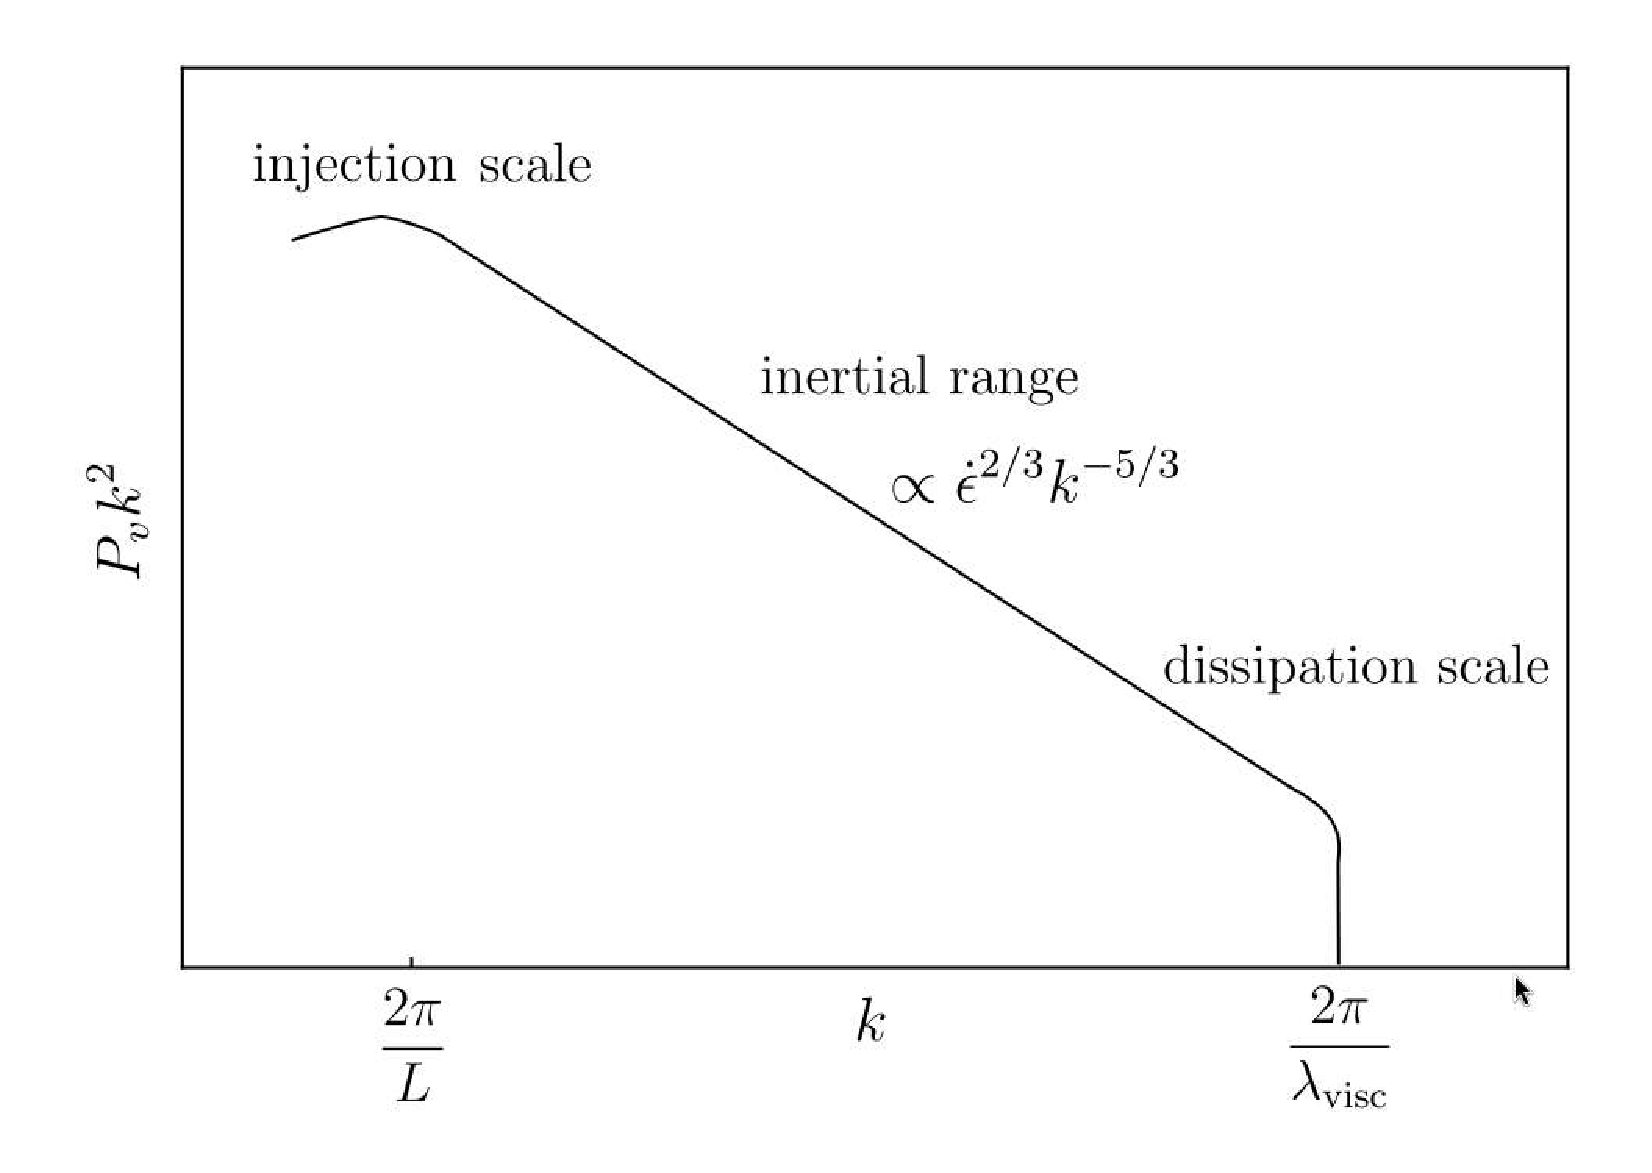
\includegraphics[width=0.852\textwidth,
	height=0.852\textheight, keepaspectratio=true]{Chapter1/imgs/tCascade.pdf}
	\caption{The turbulence cascade structure. The -5/3 value is that of omnidirectional spherical shells. If the velocity at a single point is measured over time and take a 1D Fourier transform, this would get the 1D longitudinal velocity spectrum (often denoted as $E_{11}(k_1)$). Interestingly, due to the mathematics of geometric projection, that 1D spectrum also scales as $k_1^{-5/3}$ in the inertial subrange, though with a slightly different $C_K$ pre-factor.}
		
		%The three-dimensional velocity power spectrum $P_v k^2$ as a function of wavenumber $k$, illustrating the Kolmogorov turbulent energy cascade. Energy is injected at the driving scale $2\pi/L$, transferred through the inertial range with the characteristic $\propto \dot{\epsilon}^{2/3}k^{-5/3}$ scaling, and dissipated at the viscous scale $2\pi/\lambda_\mathrm{visc}$. In the ICM context, the injection scale corresponds to the dominant	energy driver — merger shocks, sloshing, or AGN activity — while the dissipation scale is set by the effective viscosity	of the weakly collisional plasma. This is also angle averaged also known as the omnidirectional spectrum. }
	\label{Fig:3}
\end{figure}
\clearpage
%Be careful that the 5/3 is angle averaged. Versus the 11/3 is the raw 3d modal. Why we take angle averaged because it is close to what we see in measurement.

%So what the fuck are we writing here? Some more shit about turbulence? Right so sounds straight forward right? Use a telescope or spectroscopic measurement device, Observe this shit in space and constrain all the turbulence? But as people are prone to say yeah na. It is not so straightforward.

\section{Mass estimation and mass bias}

The total mass of a galaxy cluster is one of its most fundamental parameters. Along with redshift, it bridges theoretical predictions with observational data, enabling the population of galaxy clusters to act as cosmological probes \textcolor{red}{[Voit 2005, Kravtsov 2012, Allen 2011]}. Since the mass is not directly observable; it must be inferred from ICM thermodynamic properties under a set of physical assumptions. The accuracy of those assumptions --- and the systematic biases they introduce --- therefore lies at the heart of cluster cosmology.
\pbreak
Concluding this introduction is an exploration of the principal frameworks for cluster mass reconstruction, their observational implementations, and the nature of the respective biases.

\subsection{Generalized mass equation}
\label{sec:generalised_mass}

The most physically complete description of the cluster mass profile that can be obtained is acquired by integrating the full Euler equation for an inviscid collisional gas over a spherical shell \textcolor{red}{[Pratt 2019]}. Inclusive of all of the dynamical terms, the total mass enclosed within radius $r$ can be written as:

\begin{equation}
	M_{\mathrm{tot}}(<r) \;=\; M_{\mathrm{therm}} + M_{\mathrm{rand}} + M_{\mathrm{rot}}
	+ M_{\mathrm{cross}} + M_{\mathrm{stream}} + M_{\mathrm{accel}},
	\label{eq:generalised_mass}
\end{equation}
\\
where each term represents a distinct contribution to the pressure support against gravity \textcolor{red}{[Lau2013]}. The first term, $M_{\mathrm{therm}}$, is the hydrostatic mass arising from isotropic thermal pressure. The second and third terms, $M_{\mathrm{rand}}$ and $M_{\mathrm{rot}}$, account for the additional pressure support provided by turbulence and bulk gas motions, respectively. $M_{\mathrm{cross}}$, $M_{\mathrm{stream}}$, and $M_{\mathrm{accel}}$ capture contributions from cross-stream motions, bulk inflow or outflow, and local gas acceleration, all of which are more relevant during dynamically disturbed phases such as active mergers or rapid mass accretion.
\pbreak
Equation~\ref{eq:generalised_mass} is the definitive tool for numerical simulation. In a hydrodynamical simulation, all six components can be evaluated directly from three-dimensional velocity and pressure fields, providing complete knowledge of the mass budget at any radius and point of the cluster's assembly history. This makes it invaluable for quantifying the mass bias introduced by specific physical processes: sloshing cold fronts, AGN-driven cavities, merging substructure, and large-scale accretion shocks all leave distinct signatures across these terms \textcolor{red}{[Rasia2006, Nagai2007, Lau2009, Nelson2014a, Biffi2016]}. %Simulations consistently find that $M_{\mathrm{rand}}$ dominates the non-thermal correction, contributing at the level of $10$--$30\%$ of $M_\mathrm{true}$ at $R_{500}$ and growing toward the cluster outskirts, while the acceleration term $M_{\mathrm{accel}}$ becomes non-negligible only in merging systems or beyond the virial radius
\pbreak 
Despite its completeness, Equation~\ref{eq:generalised_mass} is inaccessible to direct observation. The three-dimensional velocity field cannot be confirmed from a single LOS vantage point, and even with next-generation X-ray spectroscopy \textcolor{red}{[ref]}, spatially resolved velocity will remain limited to the inner cluster regions.

%I am sorry but it is not accurate to simply call this the "Integrated" mass equation. It is an integrated value. Yes.
\subsection*{Hydrostatic mass equation}
\label{sec:he_mass}

An alternative method of acquiring radial mass estimates is from rearranging Equation \ref{eq:HE} to isolate $M(<r)$ and applying logarithmic derivatives yields:

\begin{equation}
	M_\mathrm{HSE}(<r)
	= -\frac{k_B T(r)\, r}{\mu m_p G}
	\left[
	\frac{d\ln \rho_{\mathrm{gas}}(r)}{d\ln r}
	+ \frac{d\ln T(r)}{d\ln r} 	
	\right],
	\label{eq:HE_rearrange}
\end{equation}
\\
Here $T(r)$ is the gas temperature, $\mu \approx 0.6$ is the mean molecular weight of ionised plasma, $m_p$ is the proton mass, and $G$ is the gravitational constant. This equation has been the workhorse of X-ray cluster cosmology and requires only two observationally accessible quantities where density profile $\rho_{\mathrm{gas}}(r)$, is obtained from the deprojection of X-ray surface brightness, and the temperature profile $T(r)$, obtained from spectral fitting. With the application of spatially resolved spectroscopy from \textit{XMM-Newton} and \textit{Chandra}, it has been used to derive continuous mass profiles for hundreds of clusters across a wide range of mass and redshift without requiring any assumptions about the structure of the cluster gravitational potential \textcolor{red}{[Pointecouteau 2005, Vikhlinin 2006, Ettori 2013]}. However, the weakness of this practice is also clear: it accounts only for thermal pressure support, and any residual non-thermal pressure contribution causes $M_\mathrm{HSE}$ to systematically underestimate the true mass.

\pbreak
A more complete estimate is obtained by factoring in the non-thermal pressure fraction:

\begin{equation}
	f_{\mathrm{nt}}(r) \;\equiv\; \frac{P_{\mathrm{nt}}(r)}{P_{\mathrm{tot}}(r)}
	\;=\; \frac{P_{\mathrm{nt}}(r)}{P_{\mathrm{th}}(r) + P_{\mathrm{nt}}(r)},
	\label{eq:fnt_def}
\end{equation}
\\
This introduces an additional logarithmic gradient accounting for non-thermal pressure within Equation \ref{eq:HE_rearrange} and allowing the inferred mass to be interpreted as the true enclosed mass $M_{\mathrm{true}}(<r)$. The systematic offset between the $M_{\mathrm{HSE}}(<r)$ and $M_{\mathrm{true}}(<r)$ is quantified by the \emph{hydrostatic mass bias}:

\begin{equation}
	b \;\equiv\; 1 - \frac{M_{\mathrm{HSE}}}{M_{\mathrm{true}}},
	\label{eq:mass_bias}
\end{equation}
\\
such that $b > 0$ implies an underestimate of the true mass. Under certain conditions where non-thermal pressure is the only source of bias, and assuming $f_\mathrm{nt}$ has a modestly varying radial profile, $b \approx f_{\mathrm{nt}}$. More generally, $b$ also absorbs contributions from gas temperature inhomogeneities, gas clumping, departures from spherical symmetry, and instrumental calibration uncertainties \textcolor{red}{[Rasia 2014, Pratt 2019]}. For example, a cluster with $f_{\mathrm{nt}} = 0.2$ at $R_{500}$ and a mild radial gradient, the corrected mass exceeds the purely hydrostatic value by $\sim 25\%$, broadly consistent with the range predicted by numerical simulations \textcolor{red}{[Nelson 2014a, Biffi 2016]} and inferred from  comparison of X-ray and SZ data \textcolor{red}{[Eckert 2019]}. Observationally, the bias is most directly constrained by comparing hydrostatic masses to weak gravitational lensing masses, which are free from assumptions about the gas dynamical state. Such comparisons yield values in the range $1 - b \approx 0.74$--$0.95$, with systematic differences at the $\sim 10\%$ level between different lensing programmes \textcolor{red}{[Mahdavi 2013, Hoekstra 2015, Smith 2016]}.
\newpage
%In practice, directly measuring $f_{\mathrm{nt}}(r)$ from observations remains extremely challenging. The ICM velocity field can currently be constrained only at the level of integrated line broadening in the cluster core (as demonstrated by \textit{Hitomi} for Perseus; \textcolor{red}{Hitomi2016}), and spatially resolved measurements at large radii must await the micro-calorimeter instruments aboard XRISM and Athena. In the absence of direct velocity data, $f_{\mathrm{nt}}(r)$ is commonly inferred indirectly --- by comparing hydrostatic gas fractions to the expected cosmic baryon fraction \textcolor{red}{Eckert2019}, by cross-calibrating X-ray and weak-lensing masses \textcolor{red}{Mahdavi2013, Hoekstra2015}, or by adopting theoretically motivated profiles calibrated from simulations \textcolor{red}{Nelson2014a}. Equation~\ref{eq:nt_mass} thus remains semi-empirical in current practice: its functional form is theoretically rigorous, but its application depends on externally supplied or simulation-derived estimates of $f_{\mathrm{nt}}$.


%\pbreak
%Numerical simulations are unanimous in predicting a non-zero and radially increasing hydrostatic bias. Studies consistently find $b \lesssim 5$--$10\%$ in cluster cores and $b \sim 20$--$30\%$ near $R_{500}$, with the amplitude depending strongly on dynamical state and mass accretion rate \textcolor{red}{Nagai2007, Nelson2014a, Biffi2016}. 

The mass bias carries direct consequences for cluster cosmology. Because the cluster mass function is exponentially sensitive to mass near the high-mass end, a systematic underestimate of cluster masses shifts the inferred values of $\sigma_8$ and $\Omega_m$ \textcolor{red}{[Vikhlinin 2009, Planck XX2014]}. The well-known tension between the number counts of Planck SZ-selected clusters and the primary CMB constraints on $\sigma_8$ can be partially or fully resolved by invoking a hydrostatic bias of order $b \sim 0.4$--$0.6$ \textcolor{red}{PlanckXXIV2016}, a value substantially larger than simulation predictions. Whether this discrepancy reflects unmodelled non-thermal physics, an underestimate of systematics in either probe, or new physics (e.g. a non-zero summed neutrino mass) remains an open question and is one of the primary motivations for improved cluster mass calibration.

\subsection{Mass Proxies and Scaling Relations}
\label{sec:mass_proxies}

While continuous mass equations provide physically rigorous mass profiles for individual clusters, they demand spatially resolved spectroscopic data of sufficient quality that their application is necessarily limited to a few hundred well-observed objects at most. Cosmological analyses of large cluster samples instead rely on empirically calibrated \emph{mass proxies}: global observables that correlate with mass and can be measured from lower-quality or unresolved data.

Under the simplifying assumption of self-similar gravitational collapse \textcolor{red}{Kaiser1986}, where the internal structure of virialised haloes is universal and determined only by the overdensity at formation, one expects simple power-law scaling relations between the cluster mass $M_\Delta$ and global ICM properties. Three mass proxies find particularly widespread application in X-ray and SZ-based surveys.

\subsubsection{Mass--X-ray Luminosity}
The X-ray bolometric luminosity scales with mass as
\begin{equation}
	\frac{M_{500}}{M_0} = A \left( \frac{L_X}{L_0} \right)^{\alpha} [E(z)]^{\beta},
	\label{eq:Lx_mass}
\end{equation}
\\
where $E(z) = H(z)/H_0$ encodes the self-similar redshift evolution and the expected self-similar slope is $\alpha = 3/4$ for bolometric luminosity. Because $L_X \propto n_e^2 T^{1/2} V$, the luminosity is dominated by dense core gas, making it highly sensitive to the thermodynamic state of the cluster centre. Cool-core clusters are systematically overluminous at fixed mass relative to morphologically disturbed systems, producing a large intrinsic scatter of $\sigma_{\ln M | L_X} \sim 40$--$50\%$ \textcolor{red}{Pratt2009}. The principal advantage of $L_X$ is observational accessibility: it can be measured from relatively shallow survey data with modest photon counts, making it practical for large, low signal-to-noise samples such as those from ROSAT and the forthcoming eROSITA all-sky survey.

\subsubsection{Mass--X-ray Temperature}
The spectroscopic mean temperature is related to mass via
\begin{equation}
	\frac{M_{500}}{M_0} = A \left( \frac{T_X}{T_0} \right)^{\alpha} [E(z)]^{\beta},
	\label{eq:Tx_mass}
\end{equation}
with a self-similar prediction of $\alpha = 3/2$ following from the virial theorem. $T_X$ is less susceptible to core-state bias than $L_X$ because temperature measurements are typically performed in an annular aperture that excises the central cooling region. The resulting scatter is moderate, $\sigma_{\ln M | T_X} \sim 15$--$20\%$ \textcolor{red}{Arnaud2005}, though the measurement requires significantly higher photon counts than a luminosity estimate and becomes increasingly uncertain at high redshift where spectral bins must be widened. The hydrostatic bias enters at the calibration stage, since the normalisation $A$ is typically fixed using a reference sample whose masses are derived from the HE equation.

\subsubsection{Mass--SZ Signal}
The integrated Compton-$y$ parameter, or its X-ray surrogate $Y_X = M_\mathrm{gas} T_X$ introduced by \textcolor{red}{Kravtsov2006}, scales as
\begin{equation}
	\frac{M_{500}}{M_0} = A \left( \frac{Y_{\mathrm{SZ}}}{Y_0} \right)^{\alpha} [E(z)]^{\beta},
	\label{eq:Ysz_mass}
\end{equation}
with a self-similar slope of $\alpha = 3/5$. The SZ signal is proportional to the total thermal energy of the ICM, $Y_{\mathrm{SZ}} \propto \int P_{\mathrm{th}}\, dV$, and is therefore a direct in-situ calorimeter of the gravitational potential energy deposited into the gas. Crucially, $Y_{\mathrm{SZ}}$ is insensitive to density inhomogeneities (it is linear in $n_e$ rather than quadratic), and the pressure profiles beyond the cluster core are largely governed by the depth of the gravitational potential rather than by the gas physics of the centre. This makes $Y_{\mathrm{SZ}}$ the lowest-scatter mass proxy currently available, with $\sigma_{\ln M | Y_\mathrm{SZ}} \lesssim 10\%$ in ideal conditions \textcolor{red}{daSilva2004, Motl2005, Kravtsov2006, Pike2014}. The practical limitations are the sensitivity and angular resolution of SZ instrumentation: at the resolution of \textit{Planck} ($\theta_\mathrm{FWHM} \sim 5'$), the SZ signal is significantly beam-diluted for clusters at intermediate and high redshift, requiring a clean aperture definition at $R_{500}$ or $R_{200}$ that can be difficult to establish for clusters in complex environments or without prior X-ray data.

\subsubsection{Scatter and Bias in Scaling Relations}

Each of the above proxies inherits scatter from at least three sources: intrinsic scatter in the physical relation itself (driven by the diversity of cluster formation histories and dynamical states), observational noise, and systematic biases in the mass calibration. Non-gravitational physics --- AGN feedback, cooling flows, merger-induced sloshing --- breaks the self-similar scaling at varying levels for each observable, modifying the normalisation, slope, and scatter relative to the purely gravitational prediction \textcolor{red}{LeBrun2014, Truong2018}. In particular, the slope of the $L_X$--$M$ and $Y_\mathrm{SZ}$--$M$ relations is directly affected by the mass-dependent baryon depletion discussed in Section~\ref{sec:baryon_budget}, because both $L_X$ and $Y_\mathrm{SZ}$ depend on the gas content.

A further systematic that becomes critical in the context of large cluster surveys is Malmquist/Eddington bias: because surveys select preferentially the brightest (most massive) clusters at any given noise level, the observed sample is drawn from the high-scatter tail of the intrinsic distribution. Failure to correct for this selection effect can lead to a $\sim 40\%$ underestimate of the mass at a given survey observable \textcolor{red}{Giles2017}. Properly accounting for the survey selection function in the cosmological likelihood is therefore as important as the mass calibration itself.

\begin{comment}
All about that mass no treble. So up until now we talked a lot of game on ICM physics and non thermal pressure as deviations for HE. Now we talk about their implications on mass measurements. What they are for and how non thermal pressure impact them respectively. It turns out there is multiple ways of arriving at the mass of a cluster. There are the continuous methods that elaborate mass as a function of radius $M(<r)$. This is the generalized  mass equation derived from the full Euler description of fluid:

\begin{equation}
M(<r) = M_{\mathrm{therm}} + M_{\mathrm{rand}} + M_{\mathrm{rot}} + M_{\mathrm{cross}} + M_{\mathrm{stream}} + M_{\mathrm{accel}},
\label{eq:simplifiedMass}
\end{equation}
\\
It is the simulators tool that finds its home in hydrodynamical simulation. It is awesome because we have total knowledge describing all of the component physics such as sloshing cores and AGN activity for example. We can even calculate some amount of mass bias from this:

\begin{equation}
b = 1 - \frac{M_{\mathrm{HE}}}{M_{\mathrm{true}}}
\end{equation}
\\
Despite the exacntness of the generalized $M(<r)$, it is complex (requires solving a series of non linear equations sensitive to numerical noise in simulation) and observationally blind (we can never be able to measure 3D velocity from our single vantage point on Earth). 

Another way of arriving at the $M(<r)$ relation is the integrated mass equation. It is the observers tool derived from a solution of the Jeans equation for a collisionless system of galaxies in dynamical equilibrium:

\begin{equation}
	M(<r) = -\frac{k_B T(r) r}{\mu m_p G (1 - f_{nt}(r))} \left( \frac{d \ln \rho_{gas}(r)}{d \ln r} + \frac{d \ln T(r)}{d \ln r} + \frac{d \ln (1 - f_{nt}(r))^{-1}}{d \ln r} \right)
\end{equation}
\\
It is a more simplified and practical tool that can be solved by integrating parameter data from telescopic instrumentation. However, it remains incomplete in terms of the mass bias part and relies on simplifying assumptions of spherical symmetry.

In practice both equations run complementary to each other.

\section*{Mass proxies}
While continuous equations offer a physically exact window into individual cluster dynamics, they are fundamentally limited by high data demands and observational noise. A suitable alternative can be found in a list of empirically calibrated scaling relations available in X ray and tSZ. These take an incredibly complex 3D cosmic structures and compress it into a single discrete point estimate ($M_{\mathrm{500}}$ or $M_{\mathrm{vir}}$). Quick and dirty methods for a large and expansive universe. Each of these methods are suceptible to their own scatter elements. Here are some mass proxies from X ray and tSZ. Mass versus X ray luminosity:

\begin{equation}
	%M_{\Delta} \propto \frac{1}{f_{g}}L_{X}^{\frac{3}{4}}
	\frac{M_{500}}{M_0} = A \cdot \left( \frac{L_X}{L_0} \right)^{\alpha} \cdot [E(z)]^{\beta}
\end{equation}
\\
where the expected slope for $\alpha$ is blah. It has lower barrier to entry with fewer photon counts required. These are the problems with this method (high intrinsic scatter impacted by core density anomalies such as cool core). Mass versus X ray temperature:
\begin{equation}
	%M_{\Delta} \propto T_{X}^{\frac{3}{2}}
	\frac{M_{500}}{M_0} = A \cdot \left( \frac{T_X}{T_0} \right)^{\alpha} \cdot [E(z)]^{\beta}
\end{equation}
\\
where the expected slope for $\alpha$ is blah. These are the problems with this method (moderate scatter impacted by non thermal pressure, results). Mass versus X ray temperature:

\begin{equation}
	%M_{\Delta} \propto T_{X}^{\frac{3}{2}}
	\frac{M_{500}}{M_0} = A \cdot \left( \frac{Y_{SZ}}{Y_0} \right)^{\alpha} \cdot [E(z)]^{\beta}
\end{equation}
\\
where the expected slope for $\alpha$ is blah. This method has low intrinsic scatter and is in situ thermal energy proxy which tightly tracks the total gravitational mass. These are the problems with this method. Amount of scatter (signal faint because of poor resolution large instrument beam size and requires a clean definiton of radial cutoff $R_{500}$ and $R_{200}$ the true value of which may not clear in many cases).
\end{comment}
%\begin{equation}
%	E(z) = \sqrt{\Omega_m (1+z)^3 + \Omega_\Lambda}
%\end{equation}
%%%%%%%%%%%%%%%%%%%%%%%%%%%%%%%%%%%%%%%%%%%%%%%%%%%%%%%%%%%%%%%%%%%%%%%%%%%%%%%%%%
%
% I could not find a part for this. But just keep it.
%
%%%%%%%%%%%%%%%%%%%%%%%%%%%%%%%%%%%%%%%%%%%%%%%%%%%%%%%%%%%%%%%%%%%%%%%%%%%%%%%%%%

%This is integrated mass. An additional input to get the mass estimation is the Ideal Gas law. Rearranging the HE equation gets us us the integrated mass. %The probe two different things

%\begin{equation}
%M(<r) = -\frac{k_B r}{G \mu m_p}  T(r) \left( \frac{d\ln\rho_g(r)}{d\ln r} + \frac{d\ln T(r)}{d\ln r} \right)
%\end{equation}
%\\
%Another important idea that came out of the X ray regime is beta model.

%\section{Mass cal methods}
%The abundance of clusters can be used as probes for cosmology via the cluster mass function (CMF) which has the form:

%\[ \frac{dn}{dM} = f(\sigma_{M}) \frac{ \bar{\rho}_{m}(z = 0)}{M}  \frac{d \ln \sigma_{M}^{-1}}{d M} \]

%where $\bar{\rho} (z = 0)$ is the present day mean matter density of the universe, $\sigma_{M}$ characterizes the variance of density perturbations smoothed at a given mass scale $M$, and $f(\sigma)$ describes the non-linear collapse behaviour of DM halos. Considering parameters of the \LCDM cosmology model, even small variations in cosmological parameters such as $\Omega_m$ or $\sigma_8$ may therefore induce measurable changes in the abundance of massive clusters \textcolor{red}{[ref]}. 

%In practice the inference of the CMF through empirical means is not a direct process but is often carried out through a variety of tracers that probe distinct physical components of the system. Hence the study of galaxy clusters relies on a multi spectral approach sourced from different observables each with their own unique attributes and systematics. Then we have to talk about the bias.
%\newpage
\section{Research objectives}

This work aims to take an observational approach to the ICM turbulence question. Mainly though the radio SZ angle that probe the large cluster scales. These are the main science questions framed:

\begin{itemize}
	\item What is the true nature of observable turbulence in the ICM.
	\item How much of that turbulence is observable with present instrumentation. How much will become observable with near future instrumentation?
	\item What type of improvements we can we make to remove as much bias as possible from the present methodology of turbulence inference. 
\end{itemize}

The remainder of this thesis is outlined as follows: Chapter 2 looks at the present pipeline framing the current assumptions, Chapter 3 looks at some methods we have done to interrogate those assumptions, Chapter 4 introduces a new method to circumvent some of those biases. Chapter 5 presents results and discussions.